\documentclass[a4paper, 14pt]{extarticle} %(c) we used this instead to increase the font size more than 12pt in {article}, with {extarticle} you can  
% \documentclass[a4paper, 12pt]{article}

\usepackage{fontspec, polyglossia, color}
\usepackage{amsmath, amsfonts, amssymb}
\usepackage[margin=2.5cm]{geometry}
\usepackage{float}
\usepackage{graphicx}
\usepackage{wrapfig}
\usepackage{multicol} %(c) للتقسيم لأعمدة لم استخدمها
\usepackage{hyperref}
\usepackage{url}

% \usepackage[backend=biber,style=numeric]{biblatex}
% \addbibresource{references.bib}






\setmainlanguage{arabic}
\setotherlanguage{english}
\newfontfamily\arabicfont[Script = Arabic]{Amiri}
\setmainlanguage[numerals=western]{arabic} %(c) For using Arabic numbers instead of the Indian.
\setlength{\parindent}{0pt}
\newcommand{\en}{\textenglish}
\newcommand{\s}{\strut}

%(c) For numbering the sections like 1. عنوان
% \renewcommand{\thesection}{\arabic{section}.}
%(c) For numbering the subections like (1---1).
%(c) the (---) is an em-dash and we use \textemdash cammand for it.
%(c) for an en-dash (--) use \textendash. 
\renewcommand{\thesubsection}{\arabic{section}\textemdash\arabic{subsection}}
%(c) For numbering the subsubsections like (1---1---1).
\renewcommand{\thesubsubsection}{\arabic{section}\textemdash\arabic{subsection}\textemdash\arabic{subsubsection}}



\begin{document}

  \begin{titlepage}
  \thispagestyle{empty}

  % الشعار - أعلى يسار الصفحة
  \begin{picture}(0,0)
  \put(350,-100){
\includegraphics[width=4cm]{logo.png}}
  \end{picture}

  % اسم الجامعة - أعلى يمين الصفحة
  \begin{flushleft}
    \hspace{30pt}\textbf{جامعة حلب}\\[5pt]
    \hspace{-20pt}كلية الهندسة الكهربائية والإلكترونية\\[5pt]
    قسم نظم القدرة الكهربائية
  \end{flushleft}

  \vspace{3cm}

  \begin{center}
  {\huge\bfseries التطور الحديث في محولات الاختبار عالية الجهد: المحولات الرقمية والأنظمة المعيارية}\\[1.5cm]

    \vspace{2cm}
  {\large إعداد الطالب: محمد علي قطّان \en{207047}}\\[0.5cm]
  {\large إشراف: د.عمر تميم حسن}\\[1cm]
    \vspace{2cm} 
  {\small \en{26} كانون الأول/ديسمبر \en{2025}}
  \end{center}

  \vfill
  \end{titlepage}

  \tableofcontents
  \vfill



  \section{مقدمة}
  \hspace*{10pt}
  تُعد محولات الاختبار عالية الجهد أحد أهم التجهيزات الأساسية في مختبرات التوتر العالي، حيث تُستخدم لتوليد جهود كهربائية مرتفعة بهدف اختبار متانة العوازل، وفحص مكوّنات منظومات القدرة، والتحقق من جاهزية المعدات الكهربائية قبل ربطها بالشبكات. ويقوم هذا النوع من المحولات بتحويل الجهد المنخفض من مصدر التغذية إلى جهد عالٍ مستقر يمكن التحكم به، بما يسمح بإجراء الاختبارات القياسية على المحولات، الكابلات، العوازل، وقواطع القدرة.

  ومع التطور الكبير في تقنيات القياس والتحكم خلال العقود الماضية، أصبح من الضروري تحديث محولات الاختبار التقليدية التي تعتمد عليها الكثير من المناهج والمختبرات. فالمحولات القديمة – رغم فعاليتها – تعاني من عدة قيود تتعلق بالحجم الكبير، وصعوبة المعايرة، وارتفاع مستوى المخاطر التشغيلية، إضافة إلى محدودية الدقة في القياسات. أما اليوم، فقد ظهرت محولات اختبار حديثة تعتمد على أنظمة رقمية متطورة، مما أدى إلى تحسين الأمان والدقة وسهولة التشغيل بشكل ملحوظ.

  وترتبط هذه الحلقة مباشرة بمقرر التوتر العالي الذي ندرسه حالياً، وخصوصاً الجزئية المتعلقة بمحولات الاختبار وطريقة عملها وأنواعها. إلا أنها أصبحت قديمة وقليلة الأستخدام في أوساط العمل الحالية، وهو ما يجعل دراسة التطورات الحديثة أمراً مهماً لفهم الفجوة بين التقنيات التقليدية والأنظمة المتقدمة المستخدمة حالياً في المختبرات العالمية. ومن هنا جاءت أهمية تقديم هذه الحلقة بهدف التعرف على محولات الاختبار الحديثة، وفهم كيفية تطويرها مقارنة بالأنظمة الكلاسيكية التي ندرسها في المقرر.

  \section{محولات الاختبار التقليدية}
    \subsection{تركيبها العام}
      تتكون محولات الاختبار التقليدية
      \en{(Test Transformers)}
      من بنية مشابهة للمحولات الكهربائية العادية، لكن مع بعض التعديلات لتوليد جهود عالية جداً. أهم مكونات محول الاختبار التقليدي هي:
      \begin{enumerate}
        \item \textbf{اللب الحديدي}\\
        عادةً ما يكون لب حلقي أو عمودي مصنوع من صفائح حديد سليكوني معزولة، وظيفته تجميع الفيض المغناطيسي ونقله بين الملفين.
        \item \textbf{\s
          الملف الأولي
        \en{(Primary Winding)}}\\
        يستقبل جهد التغذية المنخفض
        (
          مثلا
          $220V$
          أو
          $380V$
        ).
        عدد لفاته قليلة مقارنة بالملف الثانوي.
        \item \textbf{\s
          الملف الثانوي
          \en{(Secondary Winding)}
        }\\
        عدد لفاته كبير جداً بهدف رفع الجهد إلى قيم عالية
        (\s
          قد تصل إلى عشرات أو مئات الكيلوفولت\s
        ).
          يتم لفّ هذا الملف بعناية شديدة مع استخدام عوازل قوية تتحمل الجهد العالي.
        \item \textbf{وسط العزل الداخلي للمحول}\\
        قد يكون:\\
        زيت عازل
        (\s
        كما في المحولات التقليدية الأكبر حجماً\s
        )،\\
        أو هواء/غاز
        \en{SF6}
        في بعض الأنواع.\\
        وظيفته منع حدوث انهيار كهربائي داخل المحول.
        \item \textbf{هيكل خارجي ووصيلات جهد عالٍ}\\
        يشمل العازل الخاص بالطرف الثانوي، وغالباً يكون من البورسلان أو الإيبوكسي، بسطح طويل لمنع التفريغ.
      \end{enumerate}

    \subsection{طريقة عملها}
    محولات الاختبار تعتمد على نفس مبدأ المحولات العادية، لكنه يُستخدم هنا لرفع الجهد إلى قيم عالية لغرض الاختبار فقط.\\
    \vspace{5pt}

    آلية العمل باختصار:
    \begin{enumerate}
      \item يتم تغذية الملف الأولي بجهد منخفض.
      \item ينشأ في اللب الحديدي فيض مغناطيسي متغير.
      \item هذا الفيض يولّد قوة دافعة كهربائية في الملف الثانوي.
      \item{ 
      بسبب زيادة عدد لفات الثانوي
      \leftarrow \,
      نحصل على جهد مرتفع جداً.
      }
      \item يتم استخدام هذا الجهد العالي لاختبار:
        \begin{itemize}
          \item عوازل،
          \item كوابل،
          \item محولات قدرة،
          \item قواطع،
          \item موانع الصواعق… إلخ.
        \end{itemize}
    \end{enumerate}
    \subsection{نقاط القصور في محولات الاختبار التقليدية}
    على الرغم من موثوقيتها، إلا أن هذه المحولات تعاني من عدة مشكلات، خصوصاً عند اختبار الجهود العالية جداً:\\
    \vspace{5pt}
    
    \textbf{أولاً: الوزن الكبير}
    لتحمّل الجهود العالية، يجب زيادة:
    \begin{itemize}
      \item
      سماكة العزل الداخلي،
      \item
      حجم اللب الحديدي،
      \item 
      عدد لفات الملف الثانوي.
    \end{itemize}
    وهذا يجعل المحول ثقيل جداً وقد يصل وزنه إلى مئات الكيلوغرامات.
    
    \vspace{8pt}
    \textbf{ثانياً: الحجم الضخم}\\
    بسبب متطلبات العزل ومساحات الأمان، يكون الحجم كبيراً وغير عملي في المختبرات الصغيرة، ويتطلب عربة أو منصة خاصة لنقله.
    
    \vspace{8pt}
    \textbf{ثالثاً: صعوبة المعايرة}

    \vspace{10pt}
    معايرة محولات الاختبار التقليدية تحتاج:
    \begin{itemize}
      \item 
      تجهيزات دقيقة،
      \item 
      خبرة متقدمة،
      \item 
      ومساحة مناسبة.
    \end{itemize}
    كما تؤثر درجة الحرارة وتقدم العمر على ثبات الجهد الناتج.
    
    \vspace{8pt}
    \textbf{رابعاً: مخاطر التشغيل}

    \vspace{10pt}
    تشغيل هذه المحولات يتضمن مخاطر حقيقية بسبب الجهود العالية، مثل:
    \begin{itemize}
      \item 
      انهيار عزل فجائي يؤدي إلى شرارة أو قوس كهربائي،
      \item 
      مخاطر على المشغل إذا لم تُراعَ إجراءات السلامة،
      \item 
      احتمالية تلف العوازل أو الأجهزة قيد الاختبار.
    \end{itemize}

    
    
    % \begin{wrapfigure}{r}{0.45\textwidth}
    % \vspace{-95pt}
    % \end{wrapfigure}
    \section{محولات الاختبار الحديثة الرقمية}
    {%(c) لكي أحصل على نتائج تنسيقية أفضل عند التقسيم لأعمدة 
      \noindent %(c) هذه مالها لمزمة لأني مانع الاندنتايشن الافتراضي
      \begin{minipage}[t]{0.45\textwidth}
        \subsection{تعريفها}
      محولات الاختبار الحديثة الرقمية هي أنظمة متطورة تُستخدم لتوليد وقياس الجهود العالية في مختبرات التوتر العالي، وتعتمد بشكل أساسي على أنظمة تحكم رقمية ومعالجة رقمية للإشارات بدل الاعتماد الكامل على التحكم اليدوي والقياسات التناظرية كما في المحولات التقليدية.\\[5pt]
      تُستخدم هذه المحولات لإجراء اختبارات العزل، واختبارات الجهد المتناوب والمستمر، واختبارات الصدمات، مع مستوى أعلى من الدقة والأمان.
      \end{minipage}%
      \hfill
      \begin{minipage}[t]{0.5\textwidth}
      \begin{figure}[H]
        \vspace{-40pt} %(c) لرفع الصورة للأعلى قليلا
      \centering
      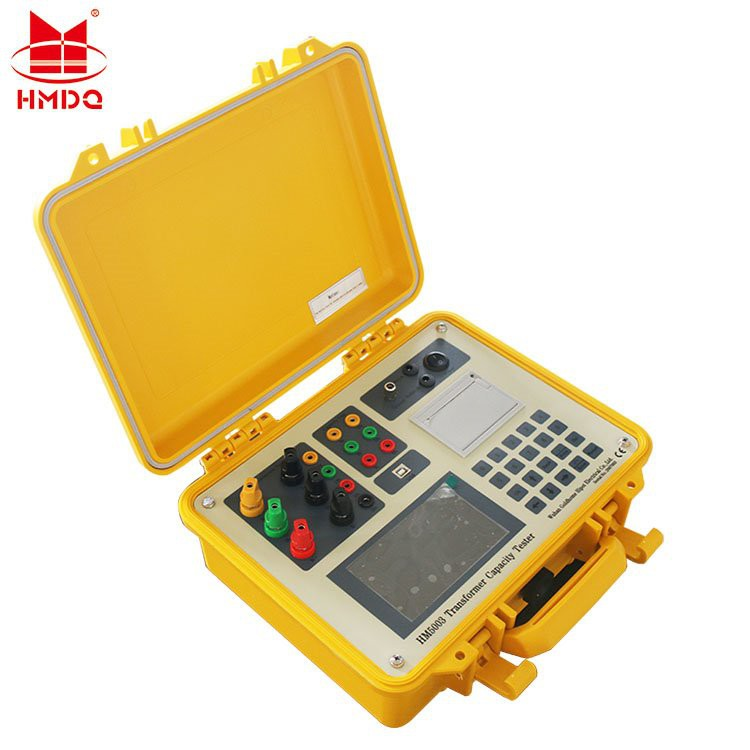
\includegraphics[width=0.70\textwidth]{transformer1.jpg}
      \caption{\en{Current Transformer CT PT Tester} — جهاز اختبارات \en{CT/PT} حديث متعدد الوظائف، يستخدم في المختبرات وميدان العمل لقياس نسبة التحويل والإثارة والقطبية وغيرها.}
      \end{figure}
      \end{minipage}
      }

      \subsection{الفروقات الأساسية بينها وبين المحولات التقليدية}
        يمكن تلخيص أهم الفروقات فيما يلي:
          \begin{itemize}
            \item 
            أسلوب التحكم:

            في المحولات التقليدية يتم التحكم برفع الجهد يدويًا، بينما في المحولات الحديثة يتم التحكم رقميًا عبر حاسوب أو واجهة تحكم إلكترونية.

            \item 
            القياس والمراقبة:

            تعتمد المحولات الحديثة على حساسات رقمية وأنظمة قياس متطورة تعطي قراءات دقيقة وفورية، على عكس القياسات التناظرية القديمة التي تتأثر بعوامل عديدة.

            \item 
            الحجم والوزن:

            المحولات الحديثة غالبًا أصغر حجمًا وأخف وزنًا نتيجة استخدام تقنيات عزل وتحكم أحدث.

            \item 
            الأمان:

            تحتوي الأنظمة الحديثة على وسائل حماية تلقائية مثل الفصل الفوري عند حدوث خلل، وهو ما يقلل من مخاطر التشغيل.

          \end{itemize}
      \subsection{نظام التحكم الرقمي}
        يعتمد نظام التحكم الرقمي في محولات الاختبار الحديثة على وحدات تحكم إلكترونية\\
        \en{(Digital Controllers)}
        متصلة بحساسات جهد وتيار دقيقة.

        يقوم النظام بـ:
          \begin{itemize}
            \item 
            التحكم التدريجي برفع وخفض الجهد بدقة عالية.
            \item 
            مراقبة قيم الجهد والتيار بشكل مستمر \en{(Real-Time)}.
            \item 
            تسجيل البيانات تلقائيًا لإمكانية تحليلها لاحقًا.
            \item 
            إيقاف النظام تلقائيًا عند تجاوز القيم المسموحة أو حدوث انهيار عزل.
          \end{itemize}
        هذا النظام يقلل الاعتماد على العامل البشري ويجعل عملية الاختبار أكثر استقرارًا وموثوقية.

        \textbf{المزايا}
        تتميز محولات الاختبار الحديثة الرقمية بعدة مزايا مهمة، من أبرزها:
        \begin{itemize}
          \item 
          دقة عالية في القياس

          بفضل الأنظمة الرقمية ومعالجة الإشارات، تكون نتائج الاختبارات أكثر دقة وأقل تأثرًا بالضوضاء والأخطاء.
          \item 
          مستوى أمان مرتفع

          توفر أنظمة الحماية الرقمية أمانًا أكبر للمشغلين والمعدات، خصوصًا في اختبارات التوتر العالي الخطرة.
          \item 
          قياسات آنية \en{(Real-Time)}

          يمكن مراقبة تغيرات الجهد والتيار أثناء الاختبار لحظة بلحظة، مما يساعد على فهم سلوك العزل بشكل أفضل.
          \item 
          تقليل الأخطاء البشرية

          التشغيل شبه الآلي يقلل من أخطاء الضبط اليدوي وسوء التقدير أثناء إجراء الاختبارات.
        \end{itemize}
    \section{الأنظمة المعيارية \en{(Modular High Voltage Test Systems)}}
      \subsection{فكرة النمط المعياري}
        تعتمد الأنظمة المعيارية لمحولات الاختبار ذات التوتر العالي على مبدأ تقسيم منظومة الاختبار إلى وحدات مستقلة \en{(Modules)}، بحيث تكون كل وحدة مسؤولة عن جزء محدد من الوظيفة الكلي
        (مثل: وحدة توليد الجهد، وحدة التحكم، وحدة القياس، وحدة الحماية).
        
        يمكن ربط هذه الوحدات معًا بحسب مستوى الجهد المطلوب أو نوع الاختبار، بدل الاعتماد على محول اختبار واحد ضخم وثابت كما في الأنظمة التقليدية.
        
        هذا المفهوم يتيح مرونة عالية في الاستخدام، حيث يمكن زيادة أو تخفيض الجهد الاختباري ببساطة عبر إضافة أو إزالة وحدات، دون الحاجة إلى تغيير المنظومة كاملة.
      \subsection{سهولة النقل والتركيب}
        من أهم ميزات الأنظمة المعيارية أنها خفيفة نسبيًا وسهلة النقل مقارنة بمحولات الاختبار التقليدية ذات الوزن والحجم الكبيرين.
        
        تُصمَّم الوحدات عادةً بحيث تكون قابلة للحمل والتركيب داخل المختبر أو حتى في مواقع العمل الميدانية.
        
        كما أن عملية التركيب لا تتطلب تجهيزات معقدة، إذ يتم توصيل الوحدات كهربائيًا وميكانيكيًا بطريقة معيارية، مما يقلل زمن الإعداد للاختبارات ويزيد من عامل الأمان أثناء التشغيل.
      \subsection{التطبيقات}
        تُستخدم الأنظمة المعيارية لمحولات الاختبار ذات التوتر العالي في مجموعة واسعة من التطبيقات، من أهمها:
        \begin{itemize}
          \item 
          اختبار \textbf{محولات القدرة}
          (اختبارات تحمل الجهد، اختبارات العزل).
          \item
          اختبار \textbf{العوازل الكهربائية}
          \en{(Porcelain, Composite Insulators)}.
          \item
          اختبار \textbf{كابلات الجهد العالي والمتوسط}.
          \item 
          اختبارات \textbf{المعامل والمختبرات التعليمية} بسبب مرونتها وسهولة التحكم بها.
        \end{itemize}
        وتُعد هذه الأنظمة مناسبة بشكل خاص للمختبرات الحديثة التي تحتاج إلى تعدد الاستخدامات دون زيادة كبيرة في الحجم أو التكلفة التشغيلية.
      
      % \begin{center} \rule{10cm}{1pt} \end{center} %(c) this for the line.
      
    \begin{figure}[H] % but this action requires to \usepackage{float}.
    \centering
    \textbf{\caption{\large جدول مقارنة مختصر بين محولات الاختبار التقليدية والأنظمة المعيارية}}
    \vspace{10pt}
    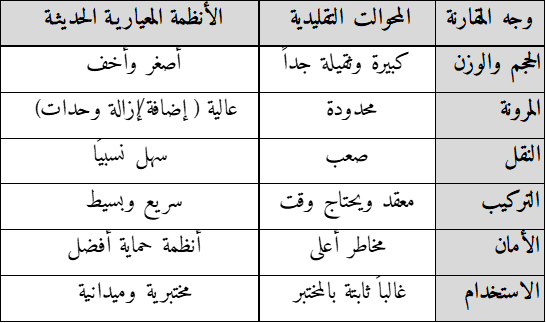
\includegraphics[width=14cm, height=8cm]{The_table.png}
    \end{figure}


    % \newpage
    \section{الخاتمة}
      في هذه الحلقة البحثية تم استعراض محولات الاختبار عالية التوتر بوصفها أحد العناصر الأساسية في مختبرات التوتر العالي، لما لها من دور مهم في توليد الجهود العالية اللازمة لاختبار العوازل والمعدات الكهربائية المختلفة. بدأنا بتعريف محولات الاختبار وبيان أهميتها، ثم تم التركيز على محولات الاختبار التقليدية من حيث تركيبها وطريقة عملها، مع توضيح أبرز نقاط القصور المرتبطة بها مثل الوزن الكبير، الحجم الضخم، صعوبة المعايرة، إضافة إلى مخاطر التشغيل والسلامة.
      
      كما تبيّن أن التطور التقني في مجال هندسة القدرة والتوتر العالي فرض الحاجة إلى تحديث محولات الاختبار لتصبح أكثر كفاءة وأمانًا، وأقل حجمًا ووزنًا، وأسهل من حيث التحكم والقياس. لذلك فإن الاتجاه الحديث في مختبرات الاختبار يميل إلى استخدام محولات اختبار مطوّرة تعتمد على تقنيات أحدث في العزل والقياس والحماية.
      
      إن دراسة هذا الموضوع ترتبط بشكل مباشر بمقرر التوتر العالي، حيث تساعد الطالب على الربط بين الجوانب النظرية والتطبيقية، وفهم التحديات العملية التي تواجه تجهيزات الاختبار في الواقع العملي. وفي الختام، يمكن القول إن تطوير محولات الاختبار يمثل خطوة أساسية لمواكبة متطلبات أنظمة القدرة الحديثة وتحسين مستوى السلامة والدقة في اختبارات الجهد العالي.
      

      \pagebreak %(c) Or you can use \newpage .

\begin{thebibliography}{} 
  \begin{LTR} %(c) We use this to make the formatting from left to right (to avoid problems).
    
    \bibitem{R1} %(c) R1 to referring to in the text by \cite{R1}. 
    \en{Wrindu,
    \textit{What Is a CT PT Tester and How Does It Work?}}\\[6pt]
    \textarabic{
    يشرح وظيفة وأهمية أجهزة اختبار محولات التيار والجهد وكيف تقيس الدقة والقطبية وغيرها.}\\[6pt]
      \en{\url{www.hvtesters.com/what-is-a-ct-pt-tester-and-how-does-it-work}}
    
    \bibitem{R2} 
    \en{DVpower,
    \textit{Current and Voltage Transformer Analyzer (CVA500)}}\\[6pt]
    \textarabic{
    مثال على جهاز اختبار حديث مع وظائف كاملة لاختبار \en{CT/PT} ودقته.}\\[6pt]
      \en{\url{www.dv-power.com/product/current-voltage-transformer-analyzer/current-and-voltage-transformer-analyzer-cva500}}
    
    \bibitem{R3} 
    \en{Megger,
    \textit{MRCT Relay and Current Transformer Test Set}}\\[6pt]
    \textarabic{مثال على جهاز اختبار تقليدي لاختبار \en{CT/VT} في المختبرات والميدان.}\\[6pt]
      \en{\url{www.megger.com/en-us/products/mrct-relay-and-current-\\
      \s transformer-test-set}}

  \end{LTR}
      
    
\end{thebibliography}



    
    
\end{document}